% Options for packages loaded elsewhere
\PassOptionsToPackage{unicode}{hyperref}
\PassOptionsToPackage{hyphens}{url}
\PassOptionsToPackage{dvipsnames,svgnames,x11names}{xcolor}
%
\documentclass[
  letterpaper,
  DIV=11,
  numbers=noendperiod]{scrartcl}

\usepackage{amsmath,amssymb}
\usepackage{iftex}
\ifPDFTeX
  \usepackage[T1]{fontenc}
  \usepackage[utf8]{inputenc}
  \usepackage{textcomp} % provide euro and other symbols
\else % if luatex or xetex
  \usepackage{unicode-math}
  \defaultfontfeatures{Scale=MatchLowercase}
  \defaultfontfeatures[\rmfamily]{Ligatures=TeX,Scale=1}
\fi
\usepackage{lmodern}
\ifPDFTeX\else  
    % xetex/luatex font selection
\fi
% Use upquote if available, for straight quotes in verbatim environments
\IfFileExists{upquote.sty}{\usepackage{upquote}}{}
\IfFileExists{microtype.sty}{% use microtype if available
  \usepackage[]{microtype}
  \UseMicrotypeSet[protrusion]{basicmath} % disable protrusion for tt fonts
}{}
\makeatletter
\@ifundefined{KOMAClassName}{% if non-KOMA class
  \IfFileExists{parskip.sty}{%
    \usepackage{parskip}
  }{% else
    \setlength{\parindent}{0pt}
    \setlength{\parskip}{6pt plus 2pt minus 1pt}}
}{% if KOMA class
  \KOMAoptions{parskip=half}}
\makeatother
\usepackage{xcolor}
\setlength{\emergencystretch}{3em} % prevent overfull lines
\setcounter{secnumdepth}{5}
% Make \paragraph and \subparagraph free-standing
\ifx\paragraph\undefined\else
  \let\oldparagraph\paragraph
  \renewcommand{\paragraph}[1]{\oldparagraph{#1}\mbox{}}
\fi
\ifx\subparagraph\undefined\else
  \let\oldsubparagraph\subparagraph
  \renewcommand{\subparagraph}[1]{\oldsubparagraph{#1}\mbox{}}
\fi

\usepackage{color}
\usepackage{fancyvrb}
\newcommand{\VerbBar}{|}
\newcommand{\VERB}{\Verb[commandchars=\\\{\}]}
\DefineVerbatimEnvironment{Highlighting}{Verbatim}{commandchars=\\\{\}}
% Add ',fontsize=\small' for more characters per line
\usepackage{framed}
\definecolor{shadecolor}{RGB}{241,243,245}
\newenvironment{Shaded}{\begin{snugshade}}{\end{snugshade}}
\newcommand{\AlertTok}[1]{\textcolor[rgb]{0.68,0.00,0.00}{#1}}
\newcommand{\AnnotationTok}[1]{\textcolor[rgb]{0.37,0.37,0.37}{#1}}
\newcommand{\AttributeTok}[1]{\textcolor[rgb]{0.40,0.45,0.13}{#1}}
\newcommand{\BaseNTok}[1]{\textcolor[rgb]{0.68,0.00,0.00}{#1}}
\newcommand{\BuiltInTok}[1]{\textcolor[rgb]{0.00,0.23,0.31}{#1}}
\newcommand{\CharTok}[1]{\textcolor[rgb]{0.13,0.47,0.30}{#1}}
\newcommand{\CommentTok}[1]{\textcolor[rgb]{0.37,0.37,0.37}{#1}}
\newcommand{\CommentVarTok}[1]{\textcolor[rgb]{0.37,0.37,0.37}{\textit{#1}}}
\newcommand{\ConstantTok}[1]{\textcolor[rgb]{0.56,0.35,0.01}{#1}}
\newcommand{\ControlFlowTok}[1]{\textcolor[rgb]{0.00,0.23,0.31}{#1}}
\newcommand{\DataTypeTok}[1]{\textcolor[rgb]{0.68,0.00,0.00}{#1}}
\newcommand{\DecValTok}[1]{\textcolor[rgb]{0.68,0.00,0.00}{#1}}
\newcommand{\DocumentationTok}[1]{\textcolor[rgb]{0.37,0.37,0.37}{\textit{#1}}}
\newcommand{\ErrorTok}[1]{\textcolor[rgb]{0.68,0.00,0.00}{#1}}
\newcommand{\ExtensionTok}[1]{\textcolor[rgb]{0.00,0.23,0.31}{#1}}
\newcommand{\FloatTok}[1]{\textcolor[rgb]{0.68,0.00,0.00}{#1}}
\newcommand{\FunctionTok}[1]{\textcolor[rgb]{0.28,0.35,0.67}{#1}}
\newcommand{\ImportTok}[1]{\textcolor[rgb]{0.00,0.46,0.62}{#1}}
\newcommand{\InformationTok}[1]{\textcolor[rgb]{0.37,0.37,0.37}{#1}}
\newcommand{\KeywordTok}[1]{\textcolor[rgb]{0.00,0.23,0.31}{#1}}
\newcommand{\NormalTok}[1]{\textcolor[rgb]{0.00,0.23,0.31}{#1}}
\newcommand{\OperatorTok}[1]{\textcolor[rgb]{0.37,0.37,0.37}{#1}}
\newcommand{\OtherTok}[1]{\textcolor[rgb]{0.00,0.23,0.31}{#1}}
\newcommand{\PreprocessorTok}[1]{\textcolor[rgb]{0.68,0.00,0.00}{#1}}
\newcommand{\RegionMarkerTok}[1]{\textcolor[rgb]{0.00,0.23,0.31}{#1}}
\newcommand{\SpecialCharTok}[1]{\textcolor[rgb]{0.37,0.37,0.37}{#1}}
\newcommand{\SpecialStringTok}[1]{\textcolor[rgb]{0.13,0.47,0.30}{#1}}
\newcommand{\StringTok}[1]{\textcolor[rgb]{0.13,0.47,0.30}{#1}}
\newcommand{\VariableTok}[1]{\textcolor[rgb]{0.07,0.07,0.07}{#1}}
\newcommand{\VerbatimStringTok}[1]{\textcolor[rgb]{0.13,0.47,0.30}{#1}}
\newcommand{\WarningTok}[1]{\textcolor[rgb]{0.37,0.37,0.37}{\textit{#1}}}

\providecommand{\tightlist}{%
  \setlength{\itemsep}{0pt}\setlength{\parskip}{0pt}}\usepackage{longtable,booktabs,array}
\usepackage{calc} % for calculating minipage widths
% Correct order of tables after \paragraph or \subparagraph
\usepackage{etoolbox}
\makeatletter
\patchcmd\longtable{\par}{\if@noskipsec\mbox{}\fi\par}{}{}
\makeatother
% Allow footnotes in longtable head/foot
\IfFileExists{footnotehyper.sty}{\usepackage{footnotehyper}}{\usepackage{footnote}}
\makesavenoteenv{longtable}
\usepackage{graphicx}
\makeatletter
\def\maxwidth{\ifdim\Gin@nat@width>\linewidth\linewidth\else\Gin@nat@width\fi}
\def\maxheight{\ifdim\Gin@nat@height>\textheight\textheight\else\Gin@nat@height\fi}
\makeatother
% Scale images if necessary, so that they will not overflow the page
% margins by default, and it is still possible to overwrite the defaults
% using explicit options in \includegraphics[width, height, ...]{}
\setkeys{Gin}{width=\maxwidth,height=\maxheight,keepaspectratio}
% Set default figure placement to htbp
\makeatletter
\def\fps@figure{htbp}
\makeatother

\KOMAoption{captions}{tableheading}
\makeatletter
\@ifpackageloaded{tcolorbox}{}{\usepackage[skins,breakable]{tcolorbox}}
\@ifpackageloaded{fontawesome5}{}{\usepackage{fontawesome5}}
\definecolor{quarto-callout-color}{HTML}{909090}
\definecolor{quarto-callout-note-color}{HTML}{0758E5}
\definecolor{quarto-callout-important-color}{HTML}{CC1914}
\definecolor{quarto-callout-warning-color}{HTML}{EB9113}
\definecolor{quarto-callout-tip-color}{HTML}{00A047}
\definecolor{quarto-callout-caution-color}{HTML}{FC5300}
\definecolor{quarto-callout-color-frame}{HTML}{acacac}
\definecolor{quarto-callout-note-color-frame}{HTML}{4582ec}
\definecolor{quarto-callout-important-color-frame}{HTML}{d9534f}
\definecolor{quarto-callout-warning-color-frame}{HTML}{f0ad4e}
\definecolor{quarto-callout-tip-color-frame}{HTML}{02b875}
\definecolor{quarto-callout-caution-color-frame}{HTML}{fd7e14}
\makeatother
\makeatletter
\makeatother
\makeatletter
\makeatother
\makeatletter
\@ifpackageloaded{caption}{}{\usepackage{caption}}
\AtBeginDocument{%
\ifdefined\contentsname
  \renewcommand*\contentsname{Table of contents}
\else
  \newcommand\contentsname{Table of contents}
\fi
\ifdefined\listfigurename
  \renewcommand*\listfigurename{List of Figures}
\else
  \newcommand\listfigurename{List of Figures}
\fi
\ifdefined\listtablename
  \renewcommand*\listtablename{List of Tables}
\else
  \newcommand\listtablename{List of Tables}
\fi
\ifdefined\figurename
  \renewcommand*\figurename{Figure}
\else
  \newcommand\figurename{Figure}
\fi
\ifdefined\tablename
  \renewcommand*\tablename{Table}
\else
  \newcommand\tablename{Table}
\fi
}
\@ifpackageloaded{float}{}{\usepackage{float}}
\floatstyle{ruled}
\@ifundefined{c@chapter}{\newfloat{codelisting}{h}{lop}}{\newfloat{codelisting}{h}{lop}[chapter]}
\floatname{codelisting}{Listing}
\newcommand*\listoflistings{\listof{codelisting}{List of Listings}}
\makeatother
\makeatletter
\@ifpackageloaded{caption}{}{\usepackage{caption}}
\@ifpackageloaded{subcaption}{}{\usepackage{subcaption}}
\makeatother
\makeatletter
\@ifpackageloaded{tcolorbox}{}{\usepackage[skins,breakable]{tcolorbox}}
\makeatother
\makeatletter
\@ifundefined{shadecolor}{\definecolor{shadecolor}{rgb}{.97, .97, .97}}
\makeatother
\makeatletter
\makeatother
\makeatletter
\makeatother
\ifLuaTeX
  \usepackage{selnolig}  % disable illegal ligatures
\fi
\IfFileExists{bookmark.sty}{\usepackage{bookmark}}{\usepackage{hyperref}}
\IfFileExists{xurl.sty}{\usepackage{xurl}}{} % add URL line breaks if available
\urlstyle{same} % disable monospaced font for URLs
\hypersetup{
  pdftitle={Input -Output with R},
  pdfauthor={Kamal Romero},
  colorlinks=true,
  linkcolor={blue},
  filecolor={Maroon},
  citecolor={Blue},
  urlcolor={Blue},
  pdfcreator={LaTeX via pandoc}}

\title{Input -Output with R}
\author{Kamal Romero}
\date{2024-03-31}

\begin{document}
\maketitle
\ifdefined\Shaded\renewenvironment{Shaded}{\begin{tcolorbox}[boxrule=0pt, borderline west={3pt}{0pt}{shadecolor}, interior hidden, frame hidden, breakable, enhanced, sharp corners]}{\end{tcolorbox}}\fi

\renewcommand*\contentsname{Table of contents}
{
\hypersetup{linkcolor=}
\setcounter{tocdepth}{3}
\tableofcontents
}
\hypertarget{r-programming-language-a-very-brief-introduction}{%
\section{R programming language: A (very) brief
introduction}\label{r-programming-language-a-very-brief-introduction}}

\hypertarget{what-is-r}{%
\subsection{What Is R?}\label{what-is-r}}

The following definition is from the book
\href{https://www.oreilly.com/library/view/learning-r/9781449357160/}{Learning
R de Richard Cotton}:

``\emph{Just to confuse you, R refers to two things. There is R, the
programming language, and R, the piece of software that you use to run
programs written in R. Fortunately, most of the time it should be clear
from the context which R is being referred to.}''

``\emph{R (the language) was created in the early 1990s by Ross Ihaka
and Robert Gentleman, then both working at the University of Auckland.
It is based upon the S language that was developed at Bell Laboratories
in the 1970s, primarily by John Chambers. R (the software) is a GNU
project, reflecting its status as important free and open source
software.}''

\hypertarget{strengths-of-r}{%
\subsection{Strengths of R}\label{strengths-of-r}}

\begin{itemize}
\item
  Free and open source
\item
  Platform independent
\item
  Foster's a reproducible workflow
\item
  Active community of users and programmers making R better
\end{itemize}

\hypertarget{working-environment}{%
\subsection{Working environment}\label{working-environment}}

In this course we will use
\href{https://posit.co/download/rstudio-desktop/}{Rstudio}.

Rstudio is an IDE (integrated development environment) that works as a
graphical interface that facilitates the use of the R language.

You have a online version,
\href{https://login.rstudio.cloud/login?redirect=\%2F}{Posit cloud}

\hypertarget{r-vs-rstudio}{%
\subsection{R vs RStudio}\label{r-vs-rstudio}}

The following image and sentence is taken from the book
\href{https://moderndive.com/index.html}{Statistical Inference via Data
Science: A ModernDive into R and the Tidyverse}

\begin{figure}

{\centering 

{[}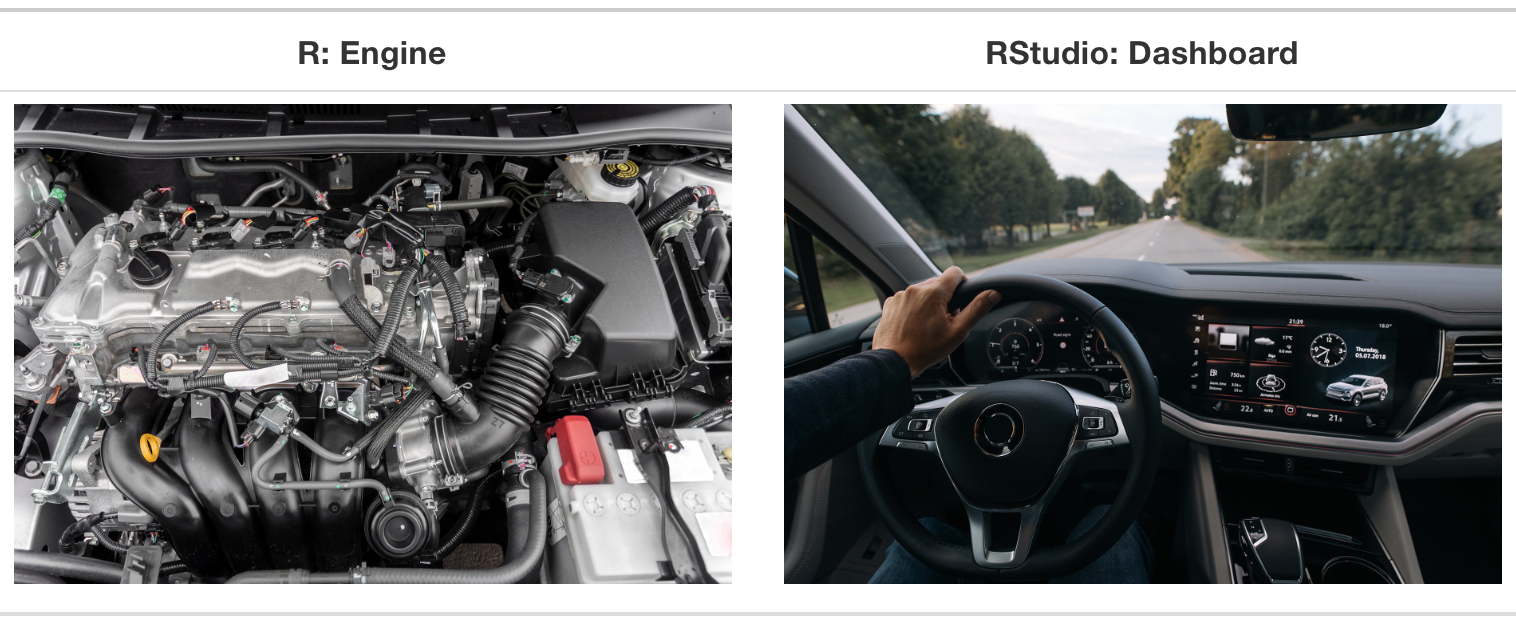
\includegraphics{IOwithR_files/mediabag/R_vs_RStudio_1.png}

}

\caption{\label{fig-rvsrstudio}\href{https://moderndive.com/1-getting-started.html}{Source}.}

\end{figure}

``\emph{More precisely, R is a programming language that runs
computations, while RStudio is an integrated development environment
(IDE) that provides an interface by adding many convenient features and
tools. So just as the way of having access to a speedometer, rearview
mirrors, and a navigation system makes driving much easier, using
RStudio's interface makes using R much easier as well.}''

\hypertarget{alternatives}{%
\subsection{Alternatives}\label{alternatives}}

There are alternatives to Rstudio, but Rstudio is the de facto R IDE for
many.

An alternative that is gaining a lot of popularity is the well-known
\href{https://code.visualstudio.com/}{Visual Studio Code}.

If you don't want to use Rstudio, this would be the suggested
alternative

\hypertarget{highlights-of-rstudio}{%
\subsection{Highlights of RStudio}\label{highlights-of-rstudio}}

\begin{figure}

{\centering 

{[}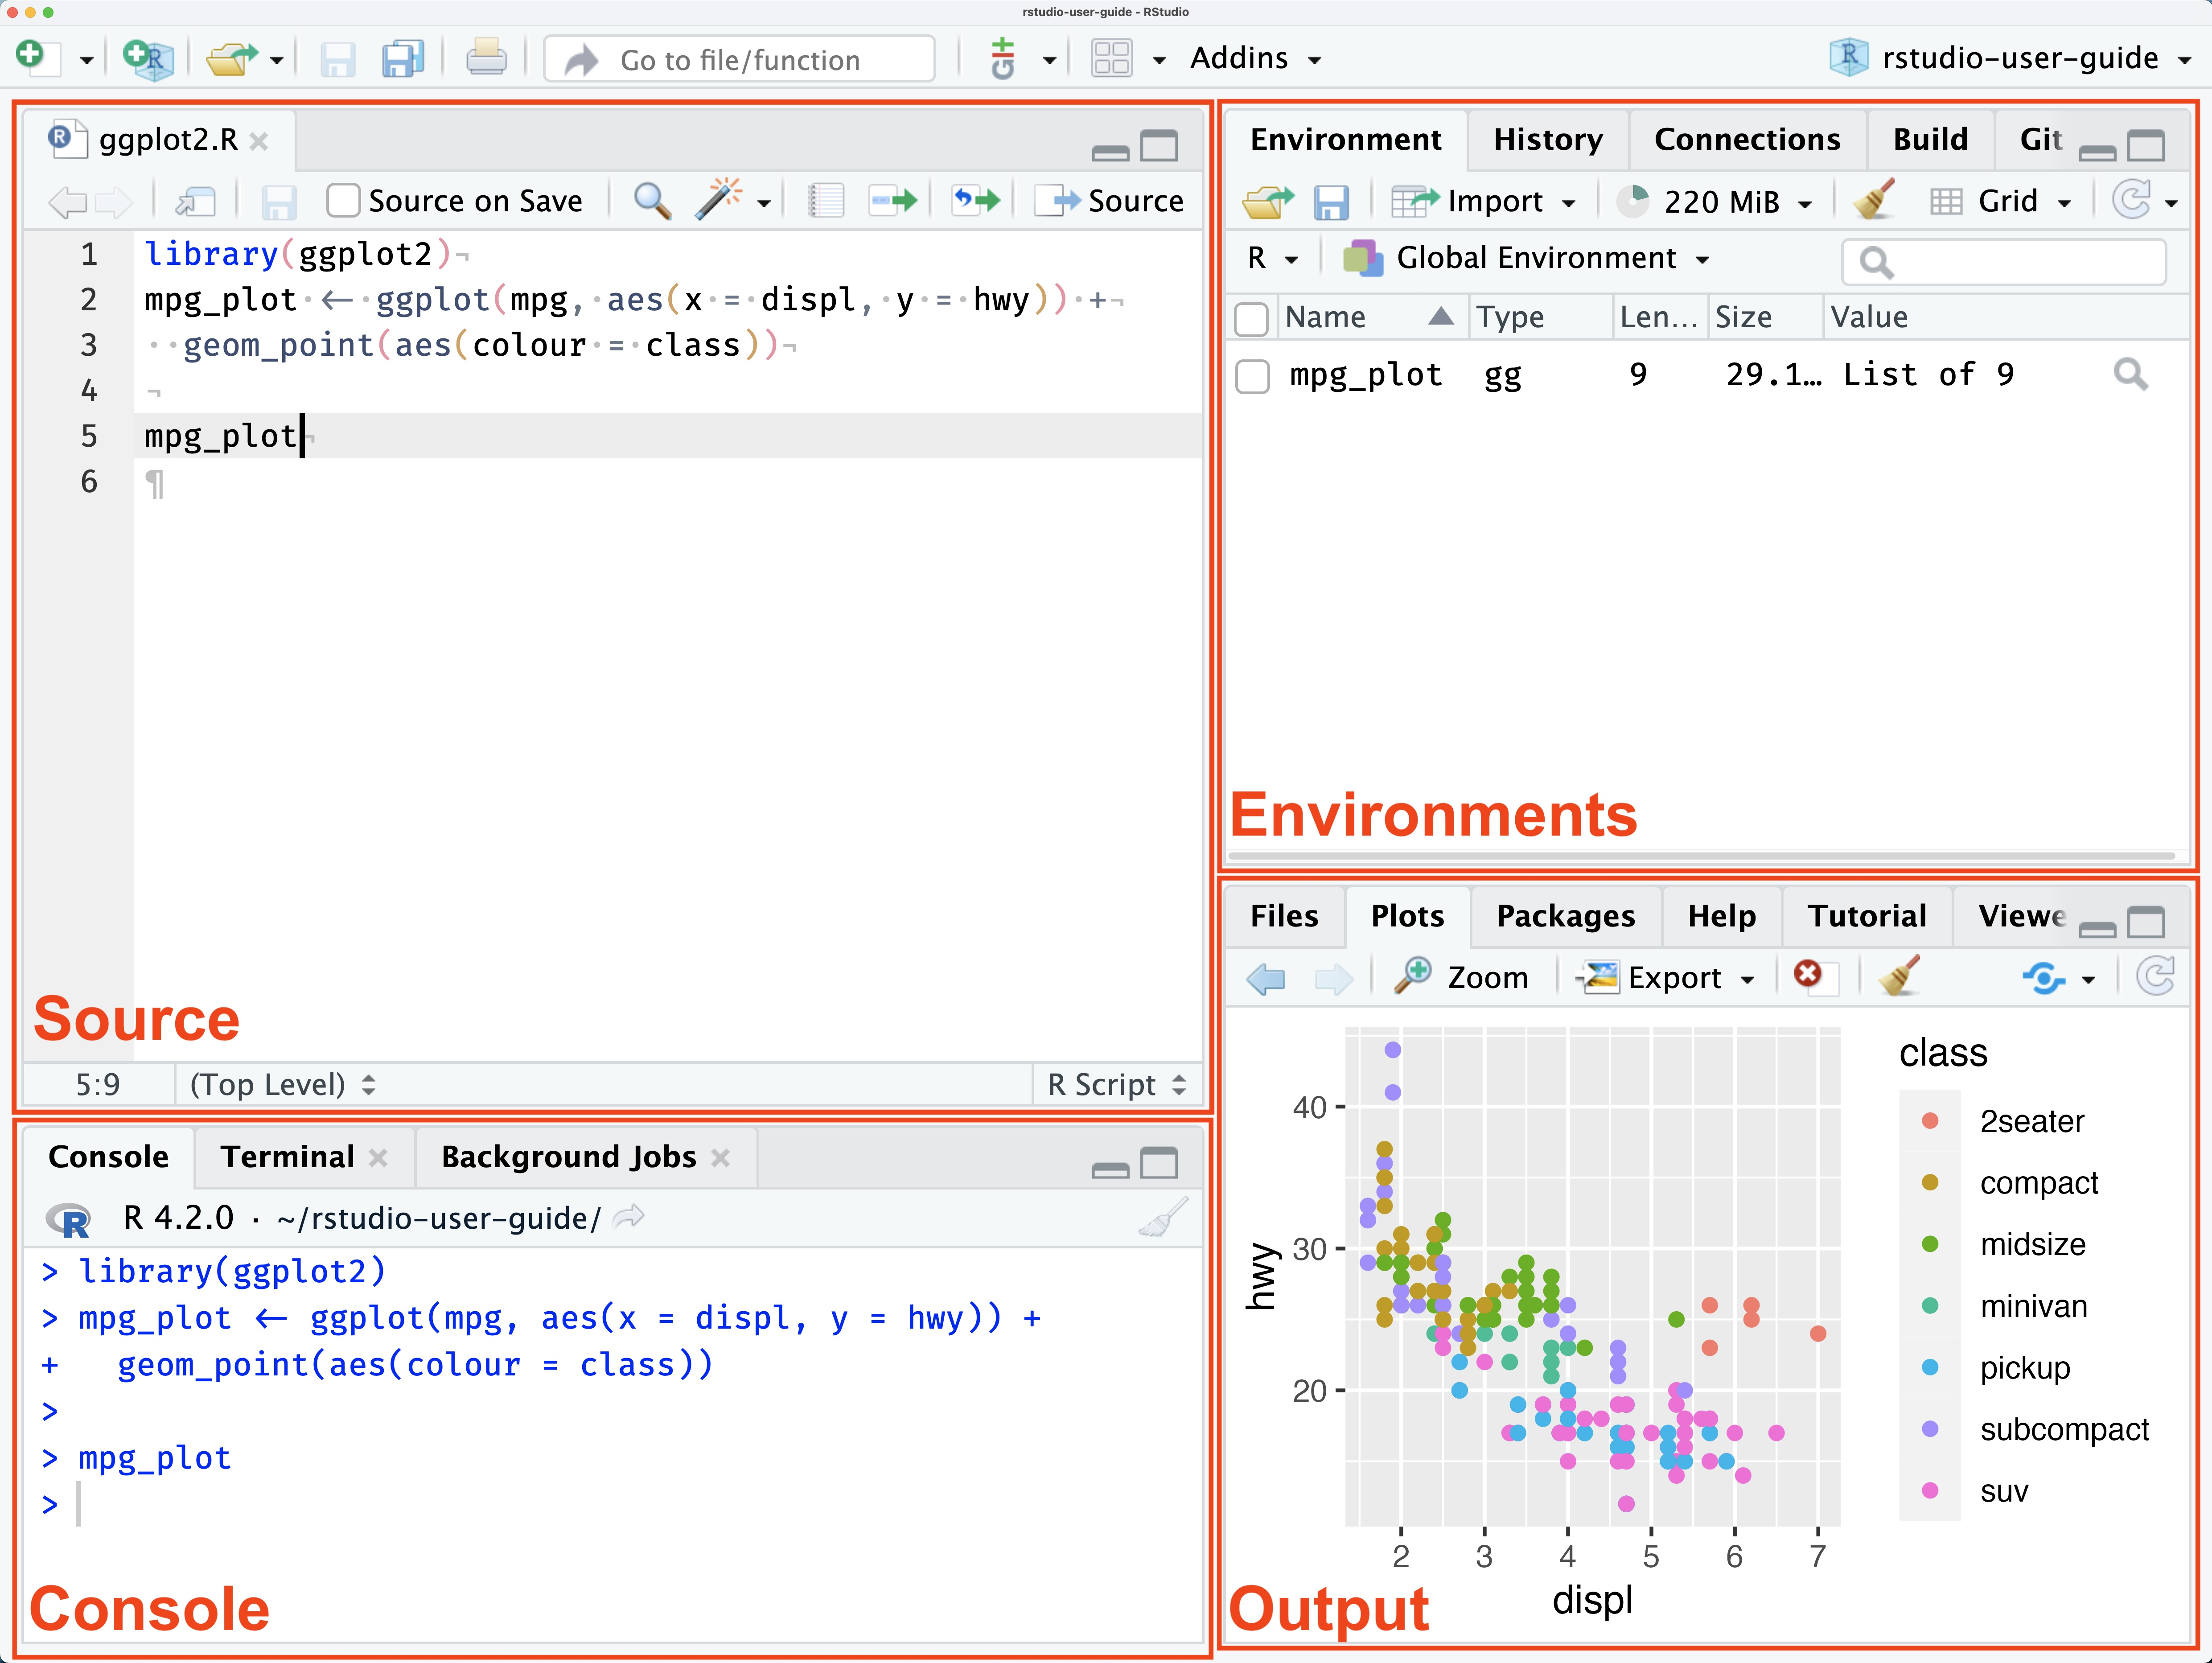
\includegraphics{images/rstudio-panes-labeled.jpeg}

}

\caption{\label{fig-rstdio}RStudio pane layout.
\href{https://docs.posit.co/ide/user/ide/guide/ui/ui-panes.html}{Source}.}

\end{figure}

\begin{itemize}
\item
  Lower Right:

  \begin{itemize}
  \tightlist
  \item
    Files, Plots, Packages, Help
  \end{itemize}
\item
  Upper Right:

  \begin{itemize}
  \tightlist
  \item
    Environment, History
  \end{itemize}
\item
  Lower Left: Console
\item
  Upper Left: Text editor
\item
  Nice Features:

  \begin{itemize}
  \tightlist
  \item
    Importing Data
  \item
    Tab completion
  \item
    \textbf{ChatGTP}
  \end{itemize}
\end{itemize}

\hypertarget{projects-directories-and-libraries-organising-the-working-environment}{%
\subsection{Projects, directories and libraries: Organising the working
environment}\label{projects-directories-and-libraries-organising-the-working-environment}}

To keep all our files organised, including databases we load or graphics
we create, we are going to work in what RStudio calls projects.

Essentially, a RStudio project is a folder or directory on your computer
that contains all the elements of your project.

\begin{figure}

{\centering 

!{[}\includegraphics{images/create RProject.gif}

}

\caption{\label{fig-project}Create a R project}

\end{figure}

The use of projects in RStudio is a good practice that allows you to
keep control of all the files used in a project.

Projects are often not only complex but also dynamic, and the management
of all the elements that make up a project is often an essential part of
the workflow.

Furthermore, the organisation into projects facilitates reproducibility.

For a more detailed discussion, read this
\href{https://r4ds.hadley.nz/workflow-scripts.html\#projects}{section}
of this \href{https://r4ds.hadley.nz/}{good book}.

\hypertarget{basic-functioning}{%
\subsection{Basic functioning}\label{basic-functioning}}

Next, we are going to introduce the basic handling of the working
environment, such as defining variables, making comments to the code,
etc. In this process, we will be introducing language concepts that we
will be defining in a formal way later on.

\hypertarget{arithmetic-operations}{%
\subsubsection{Arithmetic operations}\label{arithmetic-operations}}

To introduce us to the use of the editor and the command line of
Rstudio, we will start with some very basic operations

\begin{Shaded}
\begin{Highlighting}[]
\DecValTok{2} \SpecialCharTok{+} \DecValTok{2}
\end{Highlighting}
\end{Shaded}

\begin{verbatim}
[1] 4
\end{verbatim}

\begin{Shaded}
\begin{Highlighting}[]
\DecValTok{5} \SpecialCharTok{{-}} \DecValTok{3}
\end{Highlighting}
\end{Shaded}

\begin{verbatim}
[1] 2
\end{verbatim}

\begin{Shaded}
\begin{Highlighting}[]
\DecValTok{3} \SpecialCharTok{*} \DecValTok{2}
\end{Highlighting}
\end{Shaded}

\begin{verbatim}
[1] 6
\end{verbatim}

\begin{Shaded}
\begin{Highlighting}[]
\DecValTok{6} \SpecialCharTok{/} \DecValTok{3}
\end{Highlighting}
\end{Shaded}

\begin{verbatim}
[1] 2
\end{verbatim}

It is possible to apply standard association rules as well as operations
beyond the basic ones (power, logarithm, etc.)

\begin{Shaded}
\begin{Highlighting}[]
\NormalTok{(}\DecValTok{5} \SpecialCharTok{+} \DecValTok{3}\NormalTok{) }\SpecialCharTok{/} \DecValTok{4}
\end{Highlighting}
\end{Shaded}

\begin{verbatim}
[1] 2
\end{verbatim}

\begin{Shaded}
\begin{Highlighting}[]
\DecValTok{3}\SpecialCharTok{\^{}}\DecValTok{2}
\end{Highlighting}
\end{Shaded}

\begin{verbatim}
[1] 9
\end{verbatim}

\begin{Shaded}
\begin{Highlighting}[]
\FunctionTok{log}\NormalTok{(}\DecValTok{100}\NormalTok{, }\AttributeTok{base =} \DecValTok{10}\NormalTok{)}
\end{Highlighting}
\end{Shaded}

\begin{verbatim}
[1] 2
\end{verbatim}

\begin{Shaded}
\begin{Highlighting}[]
\DecValTok{5} \SpecialCharTok{\%\%} \DecValTok{3}
\end{Highlighting}
\end{Shaded}

\begin{verbatim}
[1] 2
\end{verbatim}

\begin{Shaded}
\begin{Highlighting}[]
\FunctionTok{sqrt}\NormalTok{(}\DecValTok{9}\NormalTok{)}
\end{Highlighting}
\end{Shaded}

\begin{verbatim}
[1] 3
\end{verbatim}

\hypertarget{assigning-variables}{%
\subsubsection{Assigning variables}\label{assigning-variables}}

We can store \emph{values} by assigning a name to them, so that we can
access the value later.

\begin{Shaded}
\begin{Highlighting}[]
\NormalTok{x }\OtherTok{\textless{}{-}} \DecValTok{4}

\NormalTok{x}
\end{Highlighting}
\end{Shaded}

\begin{verbatim}
[1] 4
\end{verbatim}

\begin{Shaded}
\begin{Highlighting}[]
\NormalTok{y }\OtherTok{\textless{}{-}}\NormalTok{ (}\DecValTok{5} \SpecialCharTok{+} \DecValTok{3}\NormalTok{) }\SpecialCharTok{/} \DecValTok{4}

\NormalTok{y}
\end{Highlighting}
\end{Shaded}

\begin{verbatim}
[1] 2
\end{verbatim}

You create variables, or create new \emph{objects} with the
\texttt{\textless{}-} operator. You can also do this in the more
conventional way with \texttt{=} but this is not standard practice.

\begin{Shaded}
\begin{Highlighting}[]
\NormalTok{Employees }\OtherTok{\textless{}{-}} \DecValTok{150}

\NormalTok{Employees}
\end{Highlighting}
\end{Shaded}

\begin{verbatim}
[1] 150
\end{verbatim}

With names you have to respect certain conventions: they must start with
a letter and can only contain letters, numbers, \texttt{\_} and
\texttt{.}.

You are free to name variables as you like, but there are some rules of
style, for example

\begin{Shaded}
\begin{Highlighting}[]
\NormalTok{i\_use\_snake\_case}
\NormalTok{otherPeopleUseCamelCase}
\NormalTok{some.people.use.periods}
\NormalTok{Lo\_queMeSale.de.por\_AHI}
\end{Highlighting}
\end{Shaded}

\begin{figure}

{\centering 

\begin{figure}

{\centering 

\href{https://allisonhorst.com/everything-else}{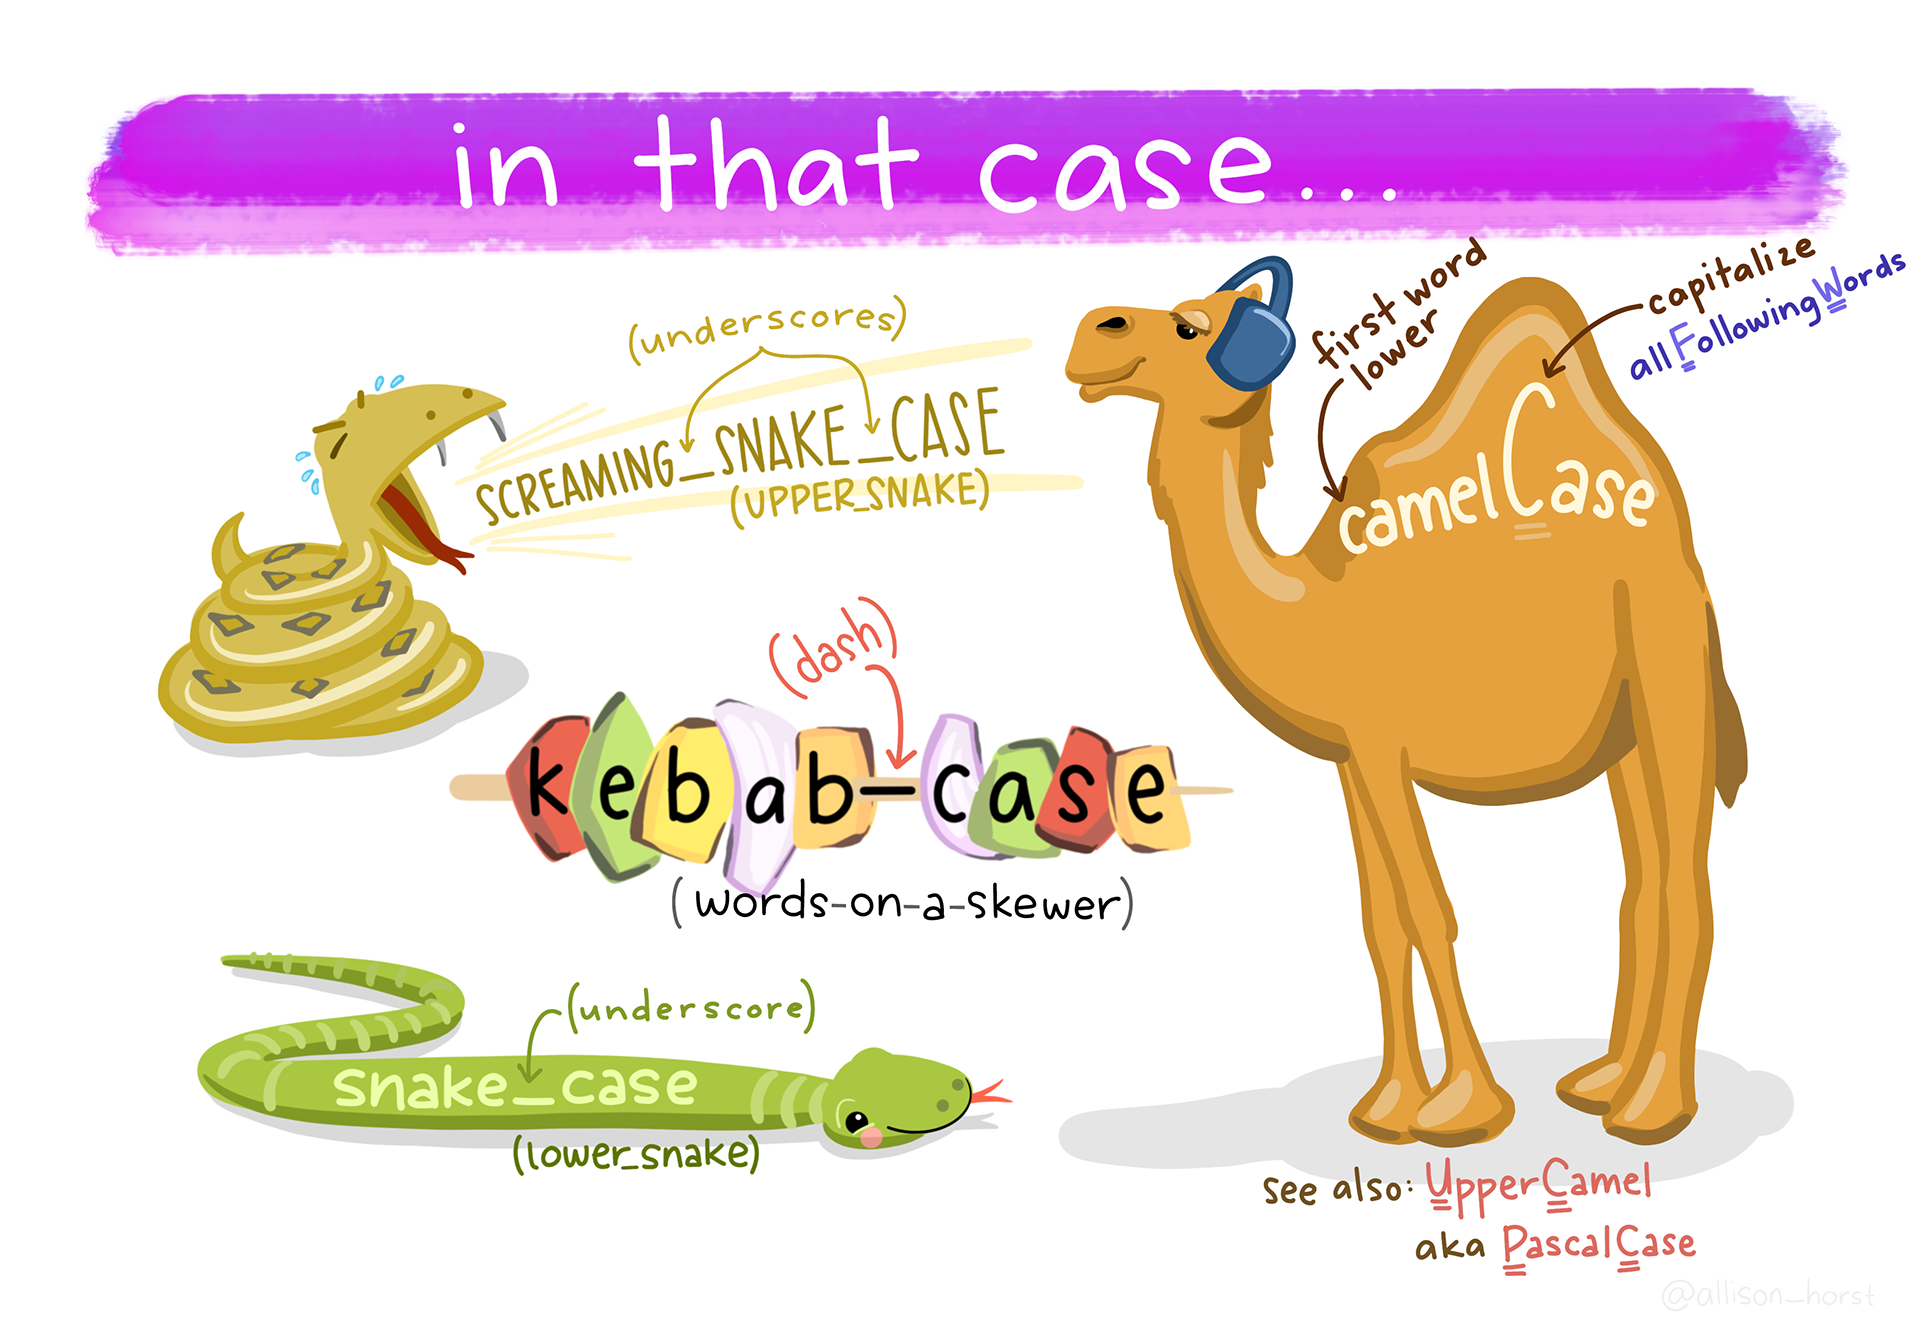
\includegraphics{IOwithR_files/mediabag/dbb99049-2916-4bc8-8.png}}

}

\end{figure}

}

\caption{\label{fig-style}An illustration of variable naming styles by
the great \href{https://allisonhorst.com/allison-horst}{Allison Horst}.
\href{https://allisonhorst.com/everything-else}{Source}.}

\end{figure}

\begin{Shaded}
\begin{Highlighting}[]
\NormalTok{New\_analysts\_January }\OtherTok{\textless{}{-}} \DecValTok{5}

\NormalTok{New\_analysts\_February }\OtherTok{\textless{}{-}} \DecValTok{3}

\NormalTok{Analysts }\OtherTok{\textless{}{-}}\NormalTok{ New\_analysts\_January }\SpecialCharTok{+}\NormalTok{ New\_analysts\_February}

\NormalTok{Analysts}
\end{Highlighting}
\end{Shaded}

\begin{verbatim}
[1] 8
\end{verbatim}

\hypertarget{introduce-comments}{%
\subsubsection{Introduce comments}\label{introduce-comments}}

Comments are initiated with

\begin{Shaded}
\begin{Highlighting}[]
\DocumentationTok{\#\# Calculation of number of analysts}
\NormalTok{Analysts }\OtherTok{\textless{}{-}}\NormalTok{ New\_analysts\_January }\SpecialCharTok{+}\NormalTok{ New\_analysts\_February}

\NormalTok{Analysts}
\end{Highlighting}
\end{Shaded}

\begin{verbatim}
[1] 8
\end{verbatim}

\hypertarget{errors}{%
\subsubsection{Errors}\label{errors}}

Throughout the course we will talk about R runtime errors, but it is
worth getting used to them, as they will always be with us 😢, but they
give us a guide to solve them 😊

\begin{Shaded}
\begin{Highlighting}[]
\DocumentationTok{\#\# analyst\_number\_calculation}
\NormalTok{Analysts\_update }\OtherTok{\textless{}{-}}\NormalTok{ New\_analysts\_January }\SpecialCharTok{+}\NormalTok{ New\_analysts\_February }\SpecialCharTok{+}\NormalTok{ New\_analysts\_March}

\NormalTok{Analyst\_update}
\end{Highlighting}
\end{Shaded}

\hypertarget{libraries}{%
\subsection{Libraries}\label{libraries}}

Libraries or packages are perhaps the most commonly used elements in R
for practical work.

A formal definition of a library from the book
\href{https://r-pkgs.org/}{R Packages} by Hadley Wickham and Jennifer
Bryan is as follows:

``\emph{In R, the fundamental unit of shareable code is the package. A
package bundles together code, data, documentation, and tests, and is
easy to share with others. As of March 2023, there were over 19,000
packages available on the Comprehensive R Archive Network, or CRAN, the
public clearing house for R packages}''.

An R package is a way to share code in an organised way that expands the
possibilities of R by extending its functionality.

Libraries are installed using the \texttt{install.packages()} command,
and libraries are loaded with \texttt{library()}.

\begin{Shaded}
\begin{Highlighting}[]
\FunctionTok{install.packages}\NormalTok{(emoji)}
\FunctionTok{library}\NormalTok{(emoji)}
\end{Highlighting}
\end{Shaded}

\hypertarget{basic-types-in-r-data-types}{%
\subsection{\texorpdfstring{Basic types in R
\href{http://www.statmethods.net/input/datatypes.html}{Data
Types}}{Basic types in R Data Types}}\label{basic-types-in-r-data-types}}

In order to work with data, it is necessary to understand how data is
stored in the computer by each programming language.

The structures that store numerical information, and the way they are
accessed, differ from Python to R, or from R to other languages.

The most important family of variable types in R are vectors, which can
be classified as either atomic or list.

\begin{itemize}
\tightlist
\item
  The common data objects in R are:

  \begin{itemize}
  \tightlist
  \item
    Vectors: one dimensional array

    \begin{itemize}
    \tightlist
    \item
      Types: numeric, integer, character, factor, logical
    \end{itemize}
  \item
    Matrices: two dimensional array

    \begin{itemize}
    \tightlist
    \item
      Each column must have the same type
    \end{itemize}
  \item
    \textbf{Data Frames}: two dimensional array

    \begin{itemize}
    \tightlist
    \item
      Columns may have different types
    \end{itemize}
  \item
    Lists

    \begin{itemize}
    \tightlist
    \item
      Items don't need to be the same size.
    \end{itemize}
  \end{itemize}
\end{itemize}

The structure of atomic vectors is as follows:

\begin{figure}

{\centering 

{[}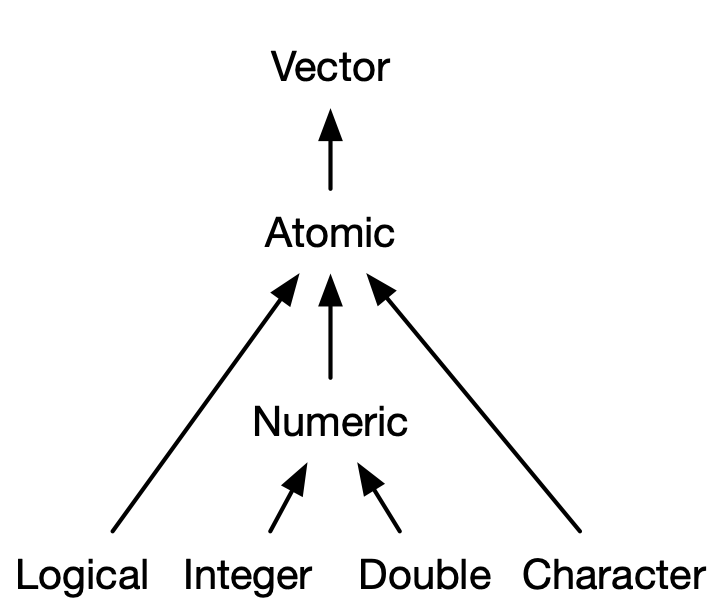
\includegraphics[width=3.125in,height=\textheight]{images/summary-tree-atomic.png}

}

\caption{\label{fig-style}Atomic vectors. Source:
\href{https://adv-r.hadley.nz/index.html}{Advanced R}}

\end{figure}

\begin{Shaded}
\begin{Highlighting}[]
\NormalTok{Number }\OtherTok{\textless{}{-}} \FloatTok{1.0} \CommentTok{\# (real, floating)}
\NormalTok{Integer }\OtherTok{\textless{}{-}} \DecValTok{1}
\NormalTok{Character }\OtherTok{\textless{}{-}} \StringTok{"ab"}   
\NormalTok{Logical }\OtherTok{\textless{}{-}} \ConstantTok{TRUE}  

\NormalTok{Number}
\end{Highlighting}
\end{Shaded}

\begin{verbatim}
[1] 1
\end{verbatim}

\begin{Shaded}
\begin{Highlighting}[]
\NormalTok{Integer}
\end{Highlighting}
\end{Shaded}

\begin{verbatim}
[1] 1
\end{verbatim}

\begin{Shaded}
\begin{Highlighting}[]
\NormalTok{Character}
\end{Highlighting}
\end{Shaded}

\begin{verbatim}
[1] "ab"
\end{verbatim}

\begin{Shaded}
\begin{Highlighting}[]
\NormalTok{Logical}
\end{Highlighting}
\end{Shaded}

\begin{verbatim}
[1] TRUE
\end{verbatim}

Be careful when working with different types

\begin{Shaded}
\begin{Highlighting}[]
\NormalTok{Number }\SpecialCharTok{+}\NormalTok{ Character}
\end{Highlighting}
\end{Shaded}

When we perform an operation with two different numeric types (real +
integer), R \emph{forces} (coerces) the result to the type with the
highest precision, in this case the real type.

\begin{Shaded}
\begin{Highlighting}[]
\NormalTok{Sum }\OtherTok{\textless{}{-}}\NormalTok{ Number }\SpecialCharTok{+}\NormalTok{ Integer}

\NormalTok{Sum}
\end{Highlighting}
\end{Shaded}

\begin{verbatim}
[1] 2
\end{verbatim}

\begin{Shaded}
\begin{Highlighting}[]
\FunctionTok{typeof}\NormalTok{(Sum)}
\end{Highlighting}
\end{Shaded}

\begin{verbatim}
[1] "double"
\end{verbatim}

Several things here, we've had our first approximation to a function in
R, a topic we'll explore in more detail later. Like the intuitive idea
we have of a function from high school mathematics, a function in R has
an argument (variable in parentheses) and gives us a result.

In R, functions have their name followed by parentheses, where we place
the argument variable(s): \texttt{a\_function(x)}.

The \texttt{typeof()} function tells us the type of the variable
(numeric, integer or logical).

\begin{Shaded}
\begin{Highlighting}[]
\FunctionTok{typeof}\NormalTok{(Number)}
\end{Highlighting}
\end{Shaded}

\begin{verbatim}
[1] "double"
\end{verbatim}

\begin{Shaded}
\begin{Highlighting}[]
\FunctionTok{typeof}\NormalTok{(Integer)}
\end{Highlighting}
\end{Shaded}

\begin{verbatim}
[1] "double"
\end{verbatim}

\begin{Shaded}
\begin{Highlighting}[]
\FunctionTok{typeof}\NormalTok{(Character)}
\end{Highlighting}
\end{Shaded}

\begin{verbatim}
[1] "character"
\end{verbatim}

\begin{Shaded}
\begin{Highlighting}[]
\FunctionTok{typeof}\NormalTok{(Logical)}
\end{Highlighting}
\end{Shaded}

\begin{verbatim}
[1] "logical"
\end{verbatim}

There are also specific functions to determine whether a variable is of
a specific type

\begin{Shaded}
\begin{Highlighting}[]
\FunctionTok{is.numeric}\NormalTok{(Number)}
\end{Highlighting}
\end{Shaded}

\begin{verbatim}
[1] TRUE
\end{verbatim}

\begin{Shaded}
\begin{Highlighting}[]
\FunctionTok{is.integer}\NormalTok{(Integer) }
\end{Highlighting}
\end{Shaded}

\begin{verbatim}
[1] FALSE
\end{verbatim}

\begin{Shaded}
\begin{Highlighting}[]
\FunctionTok{is.character}\NormalTok{(Character)}
\end{Highlighting}
\end{Shaded}

\begin{verbatim}
[1] TRUE
\end{verbatim}

\begin{Shaded}
\begin{Highlighting}[]
\FunctionTok{is.logical}\NormalTok{(Logical)}
\end{Highlighting}
\end{Shaded}

\begin{verbatim}
[1] TRUE
\end{verbatim}

We see that R tells us that \texttt{Integer} is not an integer, to
specify an integer we have to put a letter L at the end of the number

\begin{Shaded}
\begin{Highlighting}[]
\NormalTok{Integer\_2 }\OtherTok{\textless{}{-}}\NormalTok{ 1L}
\NormalTok{Integer\_2}
\end{Highlighting}
\end{Shaded}

\begin{verbatim}
[1] 1
\end{verbatim}

\begin{Shaded}
\begin{Highlighting}[]
\FunctionTok{is.integer}\NormalTok{(Integer\_2)}
\end{Highlighting}
\end{Shaded}

\begin{verbatim}
[1] TRUE
\end{verbatim}

\begin{Shaded}
\begin{Highlighting}[]
\FunctionTok{typeof}\NormalTok{(Integer\_2)}
\end{Highlighting}
\end{Shaded}

\begin{verbatim}
[1] "integer"
\end{verbatim}

\hypertarget{vectors}{%
\section{Vectors}\label{vectors}}

We are going to use R to analyse data and create statistical or
algorithmic models from it.

Most data is represented in \emph{tables}: spreadsheets, relational
databases, .csv files, etc.

Most statistical models use as input data in table form.

The most commonly used objects for working with tables in R are
\textbf{data frames} and other variants (tibble or data.tables for
example).

Before understanding how to work with tables, let's review the concept
of vector, which is the basic type on which data frames are built.

What characterises a vector is that it can store only data of the
\textbf{same type}.

\begin{Shaded}
\begin{Highlighting}[]
\NormalTok{vector\_numeric }\OtherTok{\textless{}{-}} \FunctionTok{c}\NormalTok{(}\DecValTok{1}\NormalTok{, }\DecValTok{10}\NormalTok{, }\DecValTok{49}\NormalTok{)}
\NormalTok{vector\_character }\OtherTok{\textless{}{-}} \FunctionTok{c}\NormalTok{(}\StringTok{"a"}\NormalTok{, }\StringTok{"b"}\NormalTok{, }\StringTok{"c"}\NormalTok{)}

\NormalTok{vector\_numeric}
\end{Highlighting}
\end{Shaded}

\begin{verbatim}
[1]  1 10 49
\end{verbatim}

\begin{Shaded}
\begin{Highlighting}[]
\NormalTok{vector\_character}
\end{Highlighting}
\end{Shaded}

\begin{verbatim}
[1] "a" "b" "c"
\end{verbatim}

Vectors are one-dimensional arrays (row or column) that can store
numbers, characters or logical variables.

As we have seen above, vectors are created with the \texttt{c()} command
where the c stands for \emph{combine}.

\textbf{DO NOT CONFUSE} this structure with vectors as elements of a
vector space (more on this later).

\begin{Shaded}
\begin{Highlighting}[]
\NormalTok{vector\_mixed }\OtherTok{\textless{}{-}} \FunctionTok{c}\NormalTok{(}\DecValTok{1}\NormalTok{,}\DecValTok{2}\NormalTok{, }\StringTok{"a"}\NormalTok{)}
\NormalTok{vector\_mixed}
\end{Highlighting}
\end{Shaded}

\begin{verbatim}
[1] "1" "2" "a"
\end{verbatim}

In the previous example we wanted to create a vector with elements of
different types, numeric and character. R has converted all the elements
to character.

If there are characters in a vector R converts all the elements to
character, if they are all numeric but of different types, R converts
them to the type with the highest precision (double). What happens with
logical vectors?

\begin{Shaded}
\begin{Highlighting}[]
\NormalTok{vector\_mixed2 }\OtherTok{\textless{}{-}} \FunctionTok{c}\NormalTok{(}\DecValTok{1}\NormalTok{,}\DecValTok{2}\NormalTok{,}\ConstantTok{TRUE}\NormalTok{)}
\NormalTok{vector\_mixed2}
\end{Highlighting}
\end{Shaded}

\begin{verbatim}
[1] 1 2 1
\end{verbatim}

\begin{Shaded}
\begin{Highlighting}[]
\FunctionTok{typeof}\NormalTok{(vector\_mixed2)}
\end{Highlighting}
\end{Shaded}

\begin{verbatim}
[1] "double"
\end{verbatim}

In this case R has converted the elements of the vector to numeric.

We observe something that later will be very useful, R has assigned to
the logical variable \texttt{TRUE} the number 1. The variable
\texttt{FALSE} has been assigned a zero.

Can we change a variable or a vector type? IF

\begin{Shaded}
\begin{Highlighting}[]
\NormalTok{vector\_numeric}
\end{Highlighting}
\end{Shaded}

\begin{verbatim}
[1]  1 10 49
\end{verbatim}

\begin{Shaded}
\begin{Highlighting}[]
\FunctionTok{as.character}\NormalTok{(vector\_numeric)}
\end{Highlighting}
\end{Shaded}

\begin{verbatim}
[1] "1"  "10" "49"
\end{verbatim}

\begin{Shaded}
\begin{Highlighting}[]
\NormalTok{logic\_vector }\OtherTok{\textless{}{-}} \FunctionTok{c}\NormalTok{(}\ConstantTok{TRUE}\NormalTok{, }\ConstantTok{FALSE}\NormalTok{)}

\NormalTok{logic\_vector}
\end{Highlighting}
\end{Shaded}

\begin{verbatim}
[1]  TRUE FALSE
\end{verbatim}

\begin{Shaded}
\begin{Highlighting}[]
\FunctionTok{as.numeric}\NormalTok{(logic\_vector)}
\end{Highlighting}
\end{Shaded}

\begin{verbatim}
[1] 1 0
\end{verbatim}

There are several functions in R that allow for changes of type

\begin{Shaded}
\begin{Highlighting}[]
\FunctionTok{as.character}\NormalTok{(logic\_vector)}
\end{Highlighting}
\end{Shaded}

\begin{verbatim}
[1] "TRUE"  "FALSE"
\end{verbatim}

There are a couple of other ways to create vectors

\begin{Shaded}
\begin{Highlighting}[]
\NormalTok{vector\_1 }\OtherTok{\textless{}{-}} \DecValTok{1}\SpecialCharTok{:}\DecValTok{5}

\NormalTok{vector\_2 }\OtherTok{\textless{}{-}} \FunctionTok{seq}\NormalTok{(}\DecValTok{1}\NormalTok{,}\DecValTok{5}\NormalTok{)}

\NormalTok{vector\_1}
\end{Highlighting}
\end{Shaded}

\begin{verbatim}
[1] 1 2 3 4 5
\end{verbatim}

\begin{Shaded}
\begin{Highlighting}[]
\NormalTok{vector\_2}
\end{Highlighting}
\end{Shaded}

\begin{verbatim}
[1] 1 2 3 4 5
\end{verbatim}

where \texttt{seq} stands for sequence

Since in this course the data we will use is external and not generated
by us, we will not go into the different ways of generating vectors. The
next box touches on this topic and is optional, you can follow the rest
of the lecture without reading it.

\begin{tcolorbox}[enhanced jigsaw, bottomtitle=1mm, colframe=quarto-callout-note-color-frame, opacitybacktitle=0.6, rightrule=.15mm, colbacktitle=quarto-callout-note-color!10!white, coltitle=black, toprule=.15mm, toptitle=1mm, arc=.35mm, left=2mm, titlerule=0mm, opacityback=0, colback=white, bottomrule=.15mm, breakable, title=\textcolor{quarto-callout-note-color}{\faInfo}\hspace{0.5em}{Note}, leftrule=.75mm]

More complex sequences can be created with the \texttt{seq()} function.

\begin{Shaded}
\begin{Highlighting}[]
\NormalTok{vector\_3 }\OtherTok{\textless{}{-}} \FunctionTok{seq}\NormalTok{(}\DecValTok{1}\NormalTok{,}\DecValTok{10}\NormalTok{, }\AttributeTok{by =} \DecValTok{2}\NormalTok{)}

\NormalTok{vector\_4 }\OtherTok{\textless{}{-}} \FunctionTok{seq}\NormalTok{(}\DecValTok{1}\NormalTok{,}\DecValTok{10}\NormalTok{, }\AttributeTok{length.out =} \DecValTok{20}\NormalTok{)}

\NormalTok{vector\_5 }\OtherTok{\textless{}{-}} \FunctionTok{seq}\NormalTok{(}\DecValTok{1}\NormalTok{,}\DecValTok{10}\NormalTok{, }\AttributeTok{along.with =}\NormalTok{ vector\_1)}

\NormalTok{vector\_3}
\end{Highlighting}
\end{Shaded}

\begin{verbatim}
[1] 1 3 5 7 9
\end{verbatim}

\begin{Shaded}
\begin{Highlighting}[]
\NormalTok{vector\_4}
\end{Highlighting}
\end{Shaded}

\begin{verbatim}
 [1]  1.000000  1.473684  1.947368  2.421053  2.894737  3.368421  3.842105
 [8]  4.315789  4.789474  5.263158  5.736842  6.210526  6.684211  7.157895
[15]  7.631579  8.105263  8.578947  9.052632  9.526316 10.000000
\end{verbatim}

\begin{Shaded}
\begin{Highlighting}[]
\NormalTok{vector\_5}
\end{Highlighting}
\end{Shaded}

\begin{verbatim}
[1]  1.00  3.25  5.50  7.75 10.00
\end{verbatim}

The elements of the vector can be assigned names

\begin{Shaded}
\begin{Highlighting}[]
\FunctionTok{names}\NormalTok{(vector\_1)}
\end{Highlighting}
\end{Shaded}

\begin{verbatim}
NULL
\end{verbatim}

\begin{Shaded}
\begin{Highlighting}[]
\NormalTok{names\_vec }\OtherTok{\textless{}{-}} \FunctionTok{c}\NormalTok{(}\StringTok{"one"}\NormalTok{, }\StringTok{"two"}\NormalTok{, }\StringTok{"three"}\NormalTok{, }\StringTok{"four"}\NormalTok{, }\StringTok{"five"}\NormalTok{)}

\FunctionTok{names}\NormalTok{(vector\_1) }\OtherTok{\textless{}{-}}\NormalTok{ names\_vec}

\FunctionTok{names}\NormalTok{(vector\_1)}
\end{Highlighting}
\end{Shaded}

\begin{verbatim}
[1] "one"   "two"   "three" "four"  "five" 
\end{verbatim}

Another command to generate sequences is \texttt{rep}.

\begin{Shaded}
\begin{Highlighting}[]
\NormalTok{repeated }\OtherTok{\textless{}{-}} \FunctionTok{rep}\NormalTok{(}\DecValTok{4}\NormalTok{,}\DecValTok{10}\NormalTok{)}

\NormalTok{repeated}
\end{Highlighting}
\end{Shaded}

\begin{verbatim}
 [1] 4 4 4 4 4 4 4 4 4 4
\end{verbatim}

We can repeat not only a value but vectors

\begin{Shaded}
\begin{Highlighting}[]
\NormalTok{repeat\_2 }\OtherTok{\textless{}{-}} \FunctionTok{rep}\NormalTok{(}\DecValTok{1}\SpecialCharTok{:}\DecValTok{4}\NormalTok{, }\DecValTok{4}\NormalTok{)}

\NormalTok{repeat\_2}
\end{Highlighting}
\end{Shaded}

\begin{verbatim}
 [1] 1 2 3 4 1 2 3 4 1 2 3 4 1 2 3 4
\end{verbatim}

\begin{Shaded}
\begin{Highlighting}[]
\NormalTok{repeat\_3 }\OtherTok{\textless{}{-}} \FunctionTok{rep}\NormalTok{(}\DecValTok{1}\SpecialCharTok{:}\DecValTok{4}\NormalTok{, }\AttributeTok{each =} \DecValTok{4}\NormalTok{)}

\NormalTok{repeat\_3}
\end{Highlighting}
\end{Shaded}

\begin{verbatim}
 [1] 1 1 1 1 2 2 2 2 3 3 3 3 4 4 4 4
\end{verbatim}

\begin{Shaded}
\begin{Highlighting}[]
\NormalTok{repeat\_4 }\OtherTok{\textless{}{-}} \FunctionTok{rep}\NormalTok{(}\DecValTok{1}\SpecialCharTok{:}\DecValTok{4}\NormalTok{, }\AttributeTok{each=}\DecValTok{2}\NormalTok{, }\AttributeTok{times=}\DecValTok{2}\NormalTok{)}

\NormalTok{repeat\_4}
\end{Highlighting}
\end{Shaded}

\begin{verbatim}
 [1] 1 1 2 2 3 3 4 4 1 1 2 2 3 3 4 4
\end{verbatim}

\begin{Shaded}
\begin{Highlighting}[]
\NormalTok{repeat\_5 }\OtherTok{\textless{}{-}} \FunctionTok{rep}\NormalTok{(}\DecValTok{1}\SpecialCharTok{:}\DecValTok{4}\NormalTok{, }\FunctionTok{c}\NormalTok{(}\DecValTok{2}\NormalTok{,}\DecValTok{3}\NormalTok{,}\DecValTok{4}\NormalTok{,}\DecValTok{5}\NormalTok{))}

\NormalTok{repeat\_5}
\end{Highlighting}
\end{Shaded}

\begin{verbatim}
 [1] 1 1 2 2 2 3 3 3 3 4 4 4 4 4
\end{verbatim}

We can also create \emph{random} vectors, i.e., realisations of a random
variable from a given distribution

\begin{Shaded}
\begin{Highlighting}[]
\NormalTok{random\_normal }\OtherTok{\textless{}{-}} \FunctionTok{rnorm}\NormalTok{(}\DecValTok{10}\NormalTok{)}

\NormalTok{random\_uniform }\OtherTok{\textless{}{-}} \FunctionTok{runif}\NormalTok{(}\DecValTok{10}\NormalTok{)}

\NormalTok{random\_normal}
\end{Highlighting}
\end{Shaded}

\begin{verbatim}
 [1]  0.1694287  0.1491590 -0.8231414  0.3288077  1.5108022 -0.6865587
 [7]  0.3150909 -2.4564501  0.7948955  1.0842688
\end{verbatim}

\begin{Shaded}
\begin{Highlighting}[]
\NormalTok{random\_uniform}
\end{Highlighting}
\end{Shaded}

\begin{verbatim}
 [1] 0.54759929 0.08198875 0.21239875 0.84439661 0.48560903 0.72690556
 [7] 0.24964557 0.55474315 0.86576091 0.69148726
\end{verbatim}

\end{tcolorbox}

Another characteristic of vectors besides their type, is their
\textbf{length} or dimension, which we can determine with the
\texttt{length()} function.

\begin{Shaded}
\begin{Highlighting}[]
\FunctionTok{length}\NormalTok{(vector\_1)}
\end{Highlighting}
\end{Shaded}

\begin{verbatim}
[1] 5
\end{verbatim}

\begin{Shaded}
\begin{Highlighting}[]
\FunctionTok{length}\NormalTok{(vector\_4)}
\end{Highlighting}
\end{Shaded}

\begin{verbatim}
[1] 20
\end{verbatim}

\begin{Shaded}
\begin{Highlighting}[]
\FunctionTok{length}\NormalTok{(repeat\_5)}
\end{Highlighting}
\end{Shaded}

\begin{verbatim}
[1] 14
\end{verbatim}



\end{document}
